\documentclass[11pt]{article}

\usepackage{acl}

\usepackage{times}
\usepackage{latexsym}
\usepackage[T1]{fontenc}
\usepackage[utf8]{inputenc}
\usepackage{microtype}
\usepackage{inconsolata}
\usepackage{graphicx}
\usepackage{booktabs}
\usepackage{multirow}
\usepackage{amsmath}
\usepackage{xspace}
\usepackage{subcaption}
\usepackage[capitalize,noabbrev]{cleveref}

\title{Exploring Graph Construction for Evidence Retrieval\\in Multi-Hop RAG}


\author{
  Hadas Yonat \\
  Tel Aviv University \\
  \texttt{hadasyonat@mail.tau.ac.il} \\\And
  Yuval Bukovsky \\
  Tel Aviv University \\
  \texttt{bukovsky@mail.tau.ac.il} \\\AND
  Mika Labin \\
  Tel Aviv University \\
  \texttt{mikalabin@mail.tau.ac.il} \\\And
  Gal Cohen \\
  Tel Aviv University \\
  \texttt{gc7@mail.tau.ac.il}
}

\begin{document}
\maketitle

\begin{abstract}
GraphRAG represents a corpus as a graph and retrieves subgraphs, but construction strategies are typically compared at a single default configuration of the retrieval algorithm, and any gap observed there is attributed to the construction choice. We show such comparisons are largely confounded by retrieved-set size. Over MultiHop-RAG under a fixed Prize-Collecting Steiner Tree (PCST) pipeline, the graph that appears most precise at default settings is simply the one returning fewest documents: controlling for size shrinks the precision spread across entity-, metadata-, semantic- and combined-graph construction from 0.034 to 0.003. Recall differences persist and follow each graph's oracle connectivity, the structural reachability of gold evidence. Random and shuffled controls indicate this recall signal is genuine: at closely matched retrieved size under 1-hop expansion, randomising structure reduces recall by roughly half or more, and under PCST the controls recover less evidence while retrieving twice as many documents. Dense retrieval nonetheless attains the highest recall throughout.
\end{abstract}

\section{Introduction}

Standard RAG retrieves documents by embedding similarity, which works when one semantically similar document answers the query but can miss evidence scattered across documents connected only through shared entities, events, or metadata. GraphRAG \citep{edge2024graphrag,peng2025graphragsurvey} encodes the corpus as a graph and retrieves subgraphs instead.

A central but underexplored question is \textit{how the graph should be constructed} --- by shared entities, shared metadata, embedding similarity, or a combination. Comparisons of these strategies are typically run at one default configuration of the retrieval algorithm, and any gap observed there is attributed to the construction choice itself.

We show this attribution is often incomplete. Precision is mechanically related to how many documents are retrieved, so a graph that induces PCST to return a smaller set looks more precise even if it is no better per document. We build four graph variants over MultiHop-RAG \citep{tang2024multihoprag} --- entity, metadata, semantic, and combined --- holding nodes and pipeline fixed while varying only how edges are constructed and represented, and evaluate before and after controlling retrieved-set size. Our contributions:

\begin{itemize}\itemsep0pt\parskip0pt
  \item Precision differences at default settings largely collapse once retrieved-set size is controlled, implying a common style of GraphRAG comparison conflates graph quality with retrieval budget.
  \item The recall differences that \textit{do} survive size control follow each graph's oracle connectivity, suggesting construction affects recall through structural reachability rather than scoring.
  \item Random-structure and shuffled-node controls show real construction carries signal beyond providing a graph-shaped scaffold for PCST.
\end{itemize}

\section{Background and Related Work}

\paragraph{Multi-hop RAG.} \citet{tang2024multihoprag} introduce MultiHop-RAG, a benchmark of English news articles with multi-hop questions and annotated supporting-evidence documents; standard retrieval often fails because evidence documents are not individually similar to the query.

\paragraph{GraphRAG.} \citet{edge2024graphrag} construct an entity knowledge graph with community summarisation. \citet{he2024gretriever} introduce G-Retriever, selecting subgraphs via PCST optimisation; \citet{hu2025grag} combine graph retrieval with textual evidence. \citet{gutierrez2024hipporag} and \citet{guo2024lightrag} instead vary the retrieval mechanism --- Personalized PageRank and dual-level retrieval --- over similarly entity-centric graphs. All fix one construction strategy and vary the algorithm; we target the same gap from the construction side. \citet{fatemi2024talkgraph} show both structure and text representation matter when graphs are encoded for LLMs, motivating our treatment of edge text as part of the representation rather than a neutral label.

\paragraph{Interpretable evidence routing.} \citet{sade2026exgraphrag} audit G-Retriever-style pipelines with an exactly decomposable encoder and report a \textit{semantic--structural mismatch}: nodes dominating the encoder's output are often structurally disconnected in the retrieved subgraph. Structural position and semantic importance may therefore be governed by separate mechanisms, motivating our focus on construction as a variable in its own right.

\paragraph{Gap.} Existing work either adopts a single construction method or assumes a predefined graph; the effect of alternative strategies under controlled conditions has not been systematically studied.

\section{Approach}

\subsection{Graph Construction Strategies}

We build four graph variants over the MultiHop-RAG knowledge base (609 documents after preprocessing). All share the same document nodes; only edges differ.

\textbf{Entity.} Documents sharing extracted named entities (person, organisation, location, facility, event, product) are linked. Mentions are normalised deterministically then fuzzy-merged at threshold 0.90, resolving near-duplicates (\textit{ARKANSAS}/\textit{Arkansas}) without false merges (\textit{Arkansas}/\textit{Kansas}). Edge text lists the shared entities.

\textbf{Metadata.} Documents are linked by cosine similarity between metadata records built from title and author fields, sparsified with mutual $k$-NN. Edge text is title-based (\texttt{Similar metadata record: \{title\_i\} and \{title\_j\}}), so metadata results reflect both metadata topology and title-based edge text.

\textbf{Semantic.} Documents are linked by cosine similarity between BAAI/bge-large-en-v1.5 (1024-dim) document embeddings, sparsified with mutual $k$-NN; edge text is likewise title-based.

\textbf{Combined.} $\text{entity} \cup \text{metadata} \cup \text{semantic}$, necessarily denser than any component and never density-matched to them --- a standing limitation for all combined results.

\subsection{Density Normalisation}

Natural densities differ sharply: in the unnormalised \textit{baseline} regime average degree spans 8.29 (metadata) to 24.63 (combined), with entity's maximum degree reaching 89. We therefore apply \textit{mutual $k$-NN sparsification} --- retaining only edges appearing in the $k$ nearest neighbours of \textbf{both} endpoints --- at $k \in \{10, 17, 25\}$. Mutual $k$-NN retains only $\approx$50\% of $k$ as realised average degree (0.48--0.61 across types and $k$), so $k$ is a density-ladder rung, not a degree target. The central comparison is $k{=}17$, auto-derived by the baseline pipeline when calibrating the entity graph rather than hand-picked.

\subsection{Retrieval Pipeline}

We use G-Retriever \citep{he2024gretriever}. Top-$K$ documents are retrieved by embedding similarity, $K$ auto-calibrated to entity-PCST's average output size (11--15 by regime). One of three conditions applies: \textbf{Dense} returns the $K$ seeds; \textbf{No-PCST} adds all 1-hop neighbours; \textbf{PCST} solves a Prize-Collecting Steiner Tree over the local subgraph, with node prizes from query--node similarity (identical across graph types, since node embeddings are fixed) and edge prizes from query--edge-text similarity (differing by type and template). Hyperparameters: $\mathrm{topk}{=}6$, $\mathrm{topk\_e}{=}5$, $\mathrm{cost\_e}{=}0.5$, and $0.25$ for combined to offset its edge density.

\textbf{Framing.} Because edge prizes derive from edge text, we compare \textit{practical graph representations}, not pure topology: entity edges use entity-name strings while semantic and metadata edges use title-based templates, so entity edges may be under-prized for reasons of wording.

\section{Experimental Setup}

\paragraph{Data and metrics.} MultiHop-RAG: 609 news articles, 2,556 multi-hop queries. Queries with no resolved gold evidence are excluded (301), leaving 2,255 evaluable across inference (816), comparison (856) and temporal (583). We report evidence recall, full-hit rate (all gold documents retrieved), precision, F1, average retrieved size, and \textbf{oracle connectivity} --- the fraction of gold document pairs directly connected by an edge, a retrieval-independent measure of structural reachability.

\paragraph{Gold-document deduplication.} 168 evaluable queries cite the same document more than once, as MultiHop-RAG attributes several evidence facts to one article. Retrieval is document-level, so we deduplicate gold documents before computing metrics; using raw list lengths made it possible to score $\mathrm{full\_hit}{=}1.0$ and $\mathrm{recall}{=}0.5$ simultaneously. The correction leaves precision, full-hit, size and counts unchanged and raises recall uniformly by $+0.016$--$0.018$, preserving between-condition comparisons.

\paragraph{Arms.} An unnormalised \textit{baseline} (diagnostic only); the three normalised regimes $k{=}10,17,25$; a PCST sensitivity sweep at $k{=}17$ varying $\mathrm{topk}$ and $\mathrm{cost\_e}$; and a random-control arm at $k{=}17$ (seed 123).

\section{Results}

\subsection{Main Retrieval Results}

\Cref{tab:main-results} reports the $k{=}17$ regime. After sparsification, entity, metadata and semantic reach similar average degrees (8.27--10.20) while combined, a union, reaches 17.75; semantic is nearly fully connected (2 components) where entity and metadata have 30 and 41 (full statistics in \Cref{sec:graph-stats}).

\begin{table}[t]
  \centering
  \small
  \resizebox{\columnwidth}{!}{%
  \begin{tabular}{llccccc c}
    \toprule
    \textbf{Graph} & \textbf{Method} & \textbf{Rec.} & \textbf{Full Hit} & \textbf{Prec.} & \textbf{F1} & \textbf{Size} & \textbf{Oracle} \\
    \midrule
    Dense & --- & \textbf{0.799} & \textbf{0.533} & 0.159 & 0.262 & 13.0 & --- \\
    \midrule
    \multirow{2}{*}{Entity}   & No-PCST & 0.761 & 0.464 & 0.156 & 0.256 & 12.79 & \multirow{2}{*}{0.487} \\
                              & PCST    & 0.705 & 0.424 & 0.170 & 0.267 & 11.75 & \\
    \midrule
    \multirow{2}{*}{Metadata} & No-PCST & 0.762 & 0.476 & 0.159 & 0.259 & 12.69 & \multirow{2}{*}{0.458} \\
                              & PCST    & 0.679 & 0.380 & 0.197 & 0.297 & 9.71  & \\
    \midrule
    \multirow{2}{*}{Semantic} & No-PCST & 0.780 & 0.492 & 0.157 & 0.258 & 12.95 & \multirow{2}{*}{0.544} \\
                              & PCST    & 0.690 & 0.408 & 0.204 & 0.308 & 9.18  & \\
    \midrule
    \multirow{2}{*}{Combined} & No-PCST & 0.782 & 0.500 & 0.157 & 0.259 & 12.98 & \multirow{2}{*}{0.695} \\
                              & PCST    & 0.710 & 0.431 & 0.191 & 0.296 & 9.89  & \\
    \bottomrule
  \end{tabular}%
  }
  \caption{Retrieval metrics, $k{=}17$, 2,255 evaluable queries; dense uses $K{=}13$. Oracle connectivity is a property of the graph, not the condition. Bold marks best recall and full-hit; we deliberately do not bold best precision (\S\ref{sec:size-control}).}
  \label{tab:main-results}
\end{table}

\paragraph{Precision at default settings tracks retrieved-set size.} The PCST precision ordering is identical in all four arms (baseline and $k{=}10,17,25$): semantic $>$ metadata $>$ combined $>$ entity, with a semantic--entity gap of 0.034 at $k{=}17$. Crucially the size ordering is the exact inverse: entity returns the most documents (11.75), semantic the fewest (9.18).

\paragraph{No graph condition exceeds dense on recall.} In all four arms dense retrieval attains higher recall than every graph PCST condition; entity No-PCST matches it exactly at $k{=}10$ (0.8168) but never exceeds it, and the only positive full-hit deltas occur at $k{=}10$ and do not replicate. This comparison is \textit{not} size-controlled --- dense retrieves $K{=}11$--$15$ seeds against $\approx$9--12 for graph PCST --- so we do not treat it as a clean verdict on dense-versus-graph retrieval.

\subsection{PCST Sensitivity and Size Control}
\label{sec:size-control}

Because precision is mechanically linked to set size, we swept PCST hyperparameters at $k{=}17$ --- edge penalties ($\mathrm{cost\_e} \in \{0.25, 0.5, 1.0\}$) and node thresholds ($\mathrm{topk} \in \{3, 6, 9\}$) --- to produce a range of retrieved sizes, then interpolated metrics at matched sizes.

\begin{figure}[t]
  \centering
  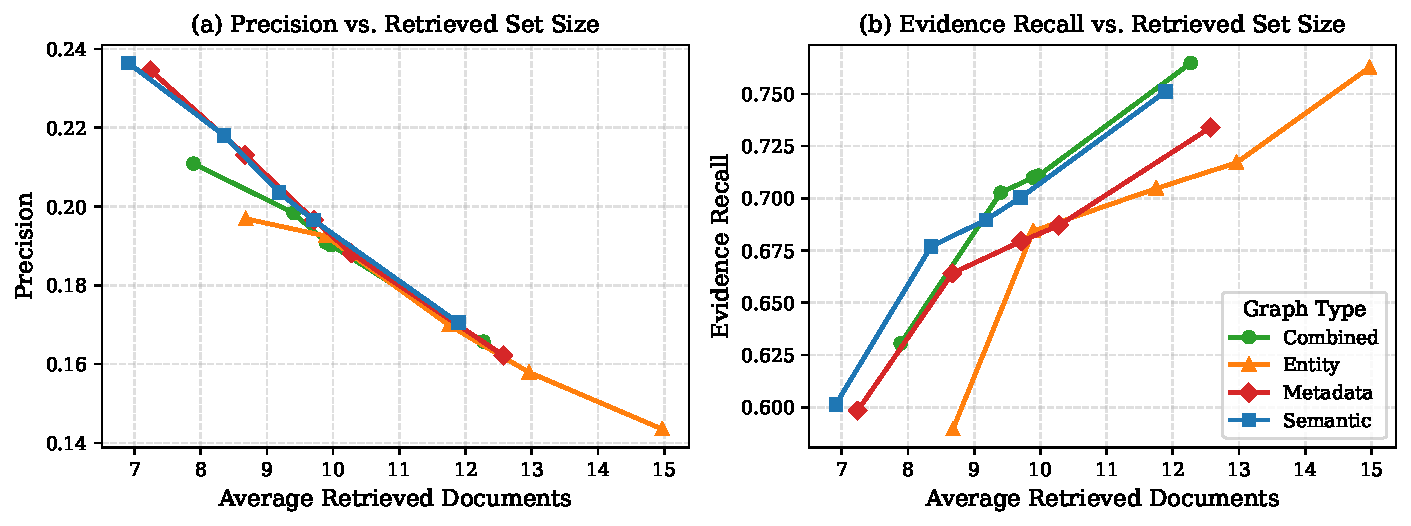
\includegraphics[width=\linewidth]{figures/fig_pcst_sensitivity.pdf}
  \caption{(a) Precision and (b) evidence recall against average retrieved size across the $k{=}17$ PCST sweep. Precision curves largely collapse at matched size; recall curves do not.}
  \label{fig:pcst-sensitivity}
\end{figure}

\begin{table}[t]
  \centering
  \small
  \begin{tabular}{lcccc}
    \toprule
    \textbf{Metric} & \textbf{Size 9} & \textbf{Size 10} & \textbf{Size 11} & \textbf{Size 11.8} \\
    \midrule
    Precision & 0.012 & \textbf{0.003} & \textbf{0.002} & \textbf{0.002} \\
    Recall    & 0.072 & 0.028          & 0.039          & 0.049          \\
    Full hit  & 0.098 & 0.048          & 0.054          & 0.059          \\
    F1        & 0.025 & 0.005          & 0.007          & 0.008          \\
    \bottomrule
  \end{tabular}
  \caption{Spread (max $-$ min) across the four graph types at matched retrieved size, interpolated from the $k{=}17$ sweep. Valid within the size overlap band 8.68--11.89.}
  \label{tab:size-control}
\end{table}

\paragraph{Precision differences collapse.} At matched size 10 the precision spread across all four types is 0.003 against 0.034 at default settings --- a $\approx$95\% reduction --- and the F1 spread is 0.005. Absent confidence intervals we report these as \textit{not distinguishable from noise} rather than as a ranking, and do not claim any strategy is the most precise.

\paragraph{Recall differences persist and follow oracle connectivity.} At matched size 10 the recall spread is 0.028, an order of magnitude larger, ordered combined (0.712) $>$ semantic (0.707) $>$ entity (0.686) $>$ metadata (0.683) --- matching the oracle-connectivity ordering (0.695 $>$ 0.544 $>$ 0.487 $>$ 0.458; \Cref{fig:oracle-vs-recall}). The correspondence rests on four graph types in one regime, where a perfect rank match has $\approx$4\% probability by chance, so we describe it as \textit{consistent with} structural reachability constraining recall, not a demonstration of it. Two measured near-matched pairs, needing no interpolation, agree: combined PCST versus entity PCST ($\mathrm{cost\_e}{=}1.0$), both at size 9.89, gives combined $+0.026$ recall and $+0.034$ full-hit with precision within 0.002; semantic PCST ($\mathrm{cost\_e}{=}0.25$, size 9.70) versus metadata PCST (size 9.71) gives identical precision (0.197) with semantic $+0.021$ recall and $+0.040$ full-hit.

\begin{figure}[t]
  \centering
  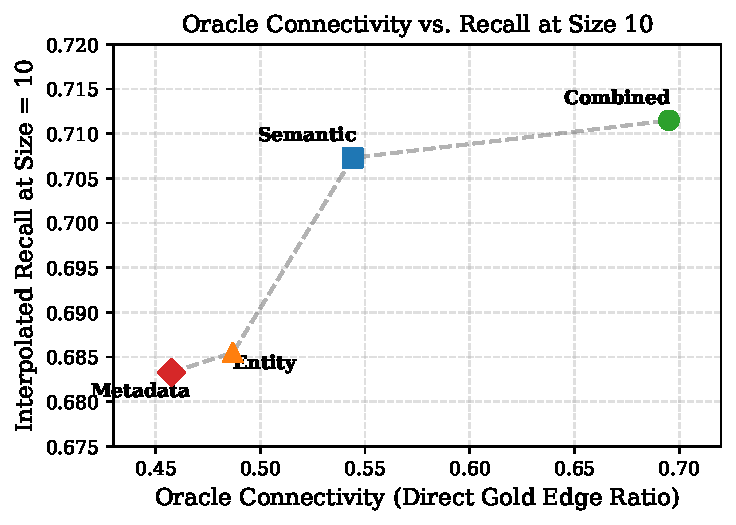
\includegraphics[width=0.85\linewidth]{figures/fig_oracle_vs_recall.pdf}
  \caption{Oracle connectivity against evidence recall interpolated at matched retrieved size 10 ($k{=}17$).}
  \label{fig:oracle-vs-recall}
\end{figure}

\subsection{Random Graph Baselines}
\label{sec:random-baselines}

To test whether real construction carries signal beyond providing a graph-shaped scaffold, we evaluate two null models at $k{=}17$ with default PCST (seed 123). \textbf{Random structure} keeps node and edge counts but rewires edges to uniformly random pairs; each random edge is assigned one of the real graph's edge attributes, so the multiset of edge attributes --- and hence the edge-prize distribution --- is preserved exactly while the endpoints it connects are randomised. \textbf{Shuffled nodes} preserves topology exactly and destroys the document--structure correspondence by permuting edge endpoints, leaving every structural statistic unchanged up to relabelling.

\begin{table}[t]
  \centering
  \small
  \resizebox{\columnwidth}{!}{%
  \begin{tabular}{lcc cc cc}
    \toprule
    & \multicolumn{2}{c}{\textbf{Real}} & \multicolumn{2}{c}{\textbf{Rand.\ struct.}} & \multicolumn{2}{c}{\textbf{Shuf.\ nodes}} \\
    \cmidrule(lr){2-3}\cmidrule(lr){4-5}\cmidrule(lr){6-7}
    \textbf{Graph} & Rec. & Size & Rec. & Size & Rec. & Size \\
    \midrule
    \multicolumn{7}{l}{\textit{No-PCST (1-hop expansion)}} \\
    Entity   & 0.761 & 12.79 & 0.396 & 12.90 & 0.245 & 9.57 \\
    Metadata & 0.762 & 12.69 & 0.396 & 12.90 & 0.397 & 12.01 \\
    Semantic & 0.780 & 12.95 & 0.242 & 10.69 & 0.244 & 10.14 \\
    Combined & 0.782 & 12.98 & 0.247 & 12.90 & 0.257 & 12.54 \\
    \midrule
    \multicolumn{7}{l}{\textit{PCST}} \\
    Entity   & 0.705 & 11.75 & 0.647 & 22.20 & 0.606 & 21.71 \\
    Metadata & 0.679 & 9.71  & 0.647 & 23.11 & 0.575 & 21.03 \\
    Semantic & 0.690 & 9.18  & 0.644 & 22.05 & 0.633 & 23.50 \\
    Combined & 0.710 & 9.89  & 0.642 & 22.78 & 0.645 & 19.53 \\
    \bottomrule
  \end{tabular}%
  }
  \caption{Real graphs versus random controls, $k{=}17$. Under No-PCST the random-structure controls are closely size-matched for entity, metadata and combined (12.7--13.0 vs 12.9); semantic and shuffled-node controls run 2--3 documents smaller, which if anything favours them. Under PCST the controls are \textit{not} size-matched, retrieving roughly twice as many documents.}
  \label{tab:random}
\end{table}

\paragraph{Under 1-hop expansion, randomising structure reduces recall by roughly half or more.} At closely matched retrieved size, real graphs reach 0.761--0.782 recall while random-structure controls reach 0.242--0.396 (\Cref{tab:random}). Full-hit rates separate even more sharply: 0.46--0.50 for real graphs against 0.003--0.118 for the eight null conditions. Expansion from dense seeds recovers supporting evidence only when edges reflect genuine document relationships.\footnote{The entity and metadata random-structure rows are identical because both graphs calibrate to the same seed size (their average degrees are 8.27 and 8.29), seeds are chosen by query--document similarity independently of the graph, and the final set is a similarity rerank; with a two-document seed and random expansion the output is dominated by the shared dense ranking. The underlying retrieval outputs differ.}

\paragraph{Under PCST the size confound runs against the controls.} The null models return substantially larger subgraphs ($\approx$19.5--23.5 documents) than real PCST ($\approx$9.2--11.8), because PCST on a random graph must reach farther to collect query-relevant nodes. A direct recall comparison is therefore size-confounded --- but in the direction that \textit{favours} the controls, so the observed gap understates the real graphs' advantage. Even with roughly twice the budget, every null condition recovers less evidence than its real counterpart (0.575--0.647 versus 0.679--0.710 recall), and null precision (0.068--0.084) is roughly 2.5$\times$ below real precision (0.170--0.204).

\section{Discussion}

\paragraph{Why semantic PCST looks most precise at default settings.} Two mechanisms combine: it returns the smallest sets (9.18 at $k{=}17$), and precision is mechanically inverse to set size at fixed relevance; semantic and metadata edges also use title-based templates, which attract higher edge prizes when titles are query-relevant. After size control the gap shrinks from 0.034 to under 0.003, so most of the apparent advantage reduces to retrieved size, and we do not conclude that semantic construction is best.

\paragraph{Why recall ordering persists.} Precision is largely a function of how many documents are returned; recall also depends on \textit{which}. Construction determines what is reachable from the seeds, and if gold evidence is not structurally reachable no scoring improvement recovers it.

\paragraph{Does construction provide genuine signal?} The controls indicate yes, for the $k{=}17$ regime tested. Shuffled nodes isolates document--topology alignment specifically: preserving every structural statistic while scrambling which documents the edges connect degrades performance to the level of the random-structure control. The specific document-to-document connections matter, not merely the presence of a graph.

\paragraph{If dense wins on recall, why use GraphRAG?} Our data do not support a recall argument, but they do support a modest compactness trade-off: graph PCST reaches recall 0.68--0.71 with 9.2--11.8 documents against dense retrieval's 0.799 with 13.0 --- a 10--29\% smaller retrieved set for a 0.09--0.12 drop in recall. Where context length, latency or cost binds this may be worthwhile, but it is a trade-off, not a free gain, and \Cref{sec:random-baselines} shows the compactness depends on the graph genuinely aligning with document relationships. We do not measure interpretability or answer quality and make no claims about them.

\section{Conclusion}

Comparing four graph construction strategies over MultiHop-RAG under a fixed G-Retriever/PCST pipeline, we find the precision differences visible at default settings are largely an artefact of retrieved-set size: controlling for size shrinks the spread by $\approx$95\%, to 0.003, which we treat as indistinguishable from noise. Recall behaves differently --- the surviving spread (0.028) is an order of magnitude larger and its ordering matches oracle connectivity, consistent with construction acting on recall through structural reachability, though we hold this as a hypothesis resting on four graph types in one regime. Random and shuffled controls indicate the recall signal is genuine rather than an artefact of having any graph to prune. Dense retrieval nonetheless attains the highest recall throughout, so we frame graph retrieval here as a compactness-versus-recall trade-off, not a recall win. The methodological takeaway: evaluations comparing construction strategies should control for retrieved-set size before attributing precision differences to graph quality.

\section*{Limitations}

\paragraph{Single-seed controls.} The null models use one seed (123). A seed sweep on shuffled-semantic oracle connectivity spans 0.003--0.029 around a density of 0.017 (seed 42 was excluded for producing connectivity 5$\times$ below density), so results are a single representative draw, not a characterisation of the null distribution.

\paragraph{Edge-attribute confound.} Edge prizes come from query--edge-text similarity, so differences between graph types may reflect wording as much as topology; entity edges lack the titles that semantic and metadata edges carry. A template-controlled ablation is left for future work.

\paragraph{No confidence intervals.} Matched-size precision and F1 differences ($\approx$0.002--0.005) are reported as collapsed, never as advantages; a query-level bootstrap would be required to assess significance.

\paragraph{Dense comparison is not size-matched.} Dense retrieves $K{=}11$--$15$ seeds against $\approx$9--12 for graph PCST, so the recall finding is confounded by size. Applying the \Cref{sec:size-control} interpolation to a dense-versus-PCST comparison is a direct extension left to future work.

\paragraph{Other.} The combined graph is a union and never density-matched, so its higher recall and connectivity may reflect density rather than complementary signal. Thresholds were calibrated then fixed, not exhaustively optimised; $\mathrm{topk\_e}$ was not varied; budget $K$ varies across regimes, confounding cross-regime recall comparisons; mutual $k$-NN retains only $\approx$50\% of $k$ as realised degree. We evaluate retrieval only --- whether retrieved sets improve generated answers, an optional goal in our proposal, was scoped out and remains untested.

\section*{Acknowledgments}

Experiments were conducted in Google Colab. All four authors contributed to data preparation, pipeline implementation, evaluation, and analysis.

\bibliography{custom}

\clearpage
\appendix

\section{Configuration}
\label{sec:config}

\begin{table}[htbp]
  \centering
  \small
  \begin{tabular}{ll}
    \toprule
    \textbf{Parameter} & \textbf{Value} \\
    \midrule
    Embedding model & BAAI/bge-large-en-v1.5 \\
    Embedding dim   & 1024 \\
    NER model       & en\_core\_web\_lg \\
    Entity types    & PERSON, ORG, GPE, LOC, \\
                    & FAC, EVENT, PRODUCT \\
    Canonicalize threshold & 0.90 \\
    Mutual $k$-NN $k$ & 10, 17, 25 \\
    PCST topk       & 6 (default) \\
    PCST topk\_e    & 5 \\
    PCST cost\_e    & 0.50 (default) \\
    PCST combined\_cost\_e & 0.25 (default) \\
    \bottomrule
  \end{tabular}
  \caption{Experiment configuration.}
  \label{tab:config}
\end{table}

\section{Graph Statistics}
\label{sec:graph-stats}

\begin{table}[htbp]
  \centering
  \small
  \begin{tabular}{lrrrr}
    \toprule
    & \textbf{Ent.} & \textbf{Meta.} & \textbf{Sem.} & \textbf{Comb.} \\
    \midrule
    Edges        & 2519 & 2525 & 3105 & 5406 \\
    Avg. degree  & 8.27 & 8.29 & 10.20 & 17.75 \\
    Max degree   & 17   & 17   & 17   & 34    \\
    Components   & 30   & 41   & 2    & 1     \\
    Largest CC   & 571  & 551  & 608  & 609   \\
    Oracle conn. & 0.487 & 0.458 & 0.544 & 0.695 \\
    \bottomrule
  \end{tabular}
  \caption{Graph statistics for the $k{=}17$ normalised regime ($n{=}609$ nodes), post-gold-dedup.}
  \label{tab:graph-stats}
\end{table}

\section{Full Results Across Regimes}
\label{sec:full-results}

\noindent The PCST hyperparameter sweep was conducted only on the $k{=}17$ regime (\Cref{sec:size-control}).

\begin{table}[htbp]
  \centering
  \small
  \resizebox{\columnwidth}{!}{%
  \begin{tabular}{llccccc}
    \toprule
    \textbf{Regime} & \textbf{Condition} & \textbf{Rec.} & \textbf{Full Hit} & \textbf{Prec.} & \textbf{F1} & \textbf{Size} \\
    \midrule
    \multirow{5}{*}{$k{=}10$}
      & Dense (no graph) & 0.817 & 0.556 & 0.141 & 0.238 & 15.0 \\
      & Entity PCST      & 0.701 & 0.414 & 0.167 & 0.261 & 12.75 \\
      & Metadata PCST    & 0.656 & 0.342 & 0.200 & 0.296 & 9.61 \\
      & Semantic PCST    & 0.683 & 0.396 & 0.212 & 0.313 & 9.17 \\
      & Combined PCST    & 0.726 & 0.444 & 0.192 & 0.298 & 10.54 \\
    \midrule
    \multirow{5}{*}{$k{=}17$}
      & Dense (no graph) & 0.799 & 0.533 & 0.159 & 0.262 & 13.0 \\
      & Entity PCST      & 0.705 & 0.424 & 0.170 & 0.267 & 11.75 \\
      & Metadata PCST    & 0.679 & 0.380 & 0.197 & 0.297 & 9.71 \\
      & Semantic PCST    & 0.690 & 0.408 & 0.204 & 0.308 & 9.18 \\
      & Combined PCST    & 0.710 & 0.431 & 0.191 & 0.296 & 9.89 \\
    \midrule
    \multirow{5}{*}{$k{=}25$}
      & Dense (no graph) & 0.783 & 0.518 & 0.168 & 0.274 & 12.0 \\
      & Entity PCST      & 0.705 & 0.424 & 0.179 & 0.278 & 10.94 \\
      & Metadata PCST    & 0.684 & 0.397 & 0.196 & 0.299 & 9.47 \\
      & Semantic PCST    & 0.685 & 0.400 & 0.201 & 0.306 & 9.05 \\
      & Combined PCST    & 0.706 & 0.424 & 0.187 & 0.291 & 9.95 \\
    \bottomrule
  \end{tabular}%
  }
  \caption{PCST metrics across the three normalised regimes at default PCST settings (2,255 evaluable queries). Cross-regime recall comparisons are confounded by differing dense seed budgets ($K{=}15, 13, 12$ for $k{=}10, 17, 25$).}
  \label{tab:full-results}
\end{table}

\section{Query-Type Breakdown}
\label{sec:qtype}

\noindent Temporal queries are consistently easiest and inference queries hardest. The graph-type ranking is stable for comparison and temporal queries, matching the aggregate ordering, but \textit{inverts} on inference queries, where metadata ranks first (0.641) and semantic last (0.620). The spread there is only 0.021, so we do not read a specialised advantage into it, but the aggregate ranking is not uniform across question types.

\begin{table}[htbp]
  \centering
  \small
  \begin{tabular}{llcc}
    \toprule
    \textbf{Graph} & \textbf{Type} & \textbf{Recall} & \textbf{Full Hit} \\
    \midrule
    \multirow{3}{*}{Entity}   & Inference  & 0.637 & 0.264 \\
                              & Comparison & 0.719 & 0.491 \\
                              & Temporal   & 0.780 & 0.552 \\
    \midrule
    \multirow{3}{*}{Metadata} & Inference  & 0.641 & 0.253 \\
                              & Comparison & 0.682 & 0.439 \\
                              & Temporal   & 0.730 & 0.472 \\
    \midrule
    \multirow{3}{*}{Semantic} & Inference  & 0.620 & 0.246 \\
                              & Comparison & 0.707 & 0.486 \\
                              & Temporal   & 0.762 & 0.521 \\
    \midrule
    \multirow{3}{*}{Combined} & Inference  & 0.635 & 0.257 \\
                              & Comparison & 0.734 & 0.522 \\
                              & Temporal   & 0.780 & 0.539 \\
    \bottomrule
  \end{tabular}
  \caption{Evidence recall and full-hit rate by question type, $k{=}17$ PCST conditions.}
  \label{tab:qtype}
\end{table}

\begin{figure}[htbp]
  \centering
  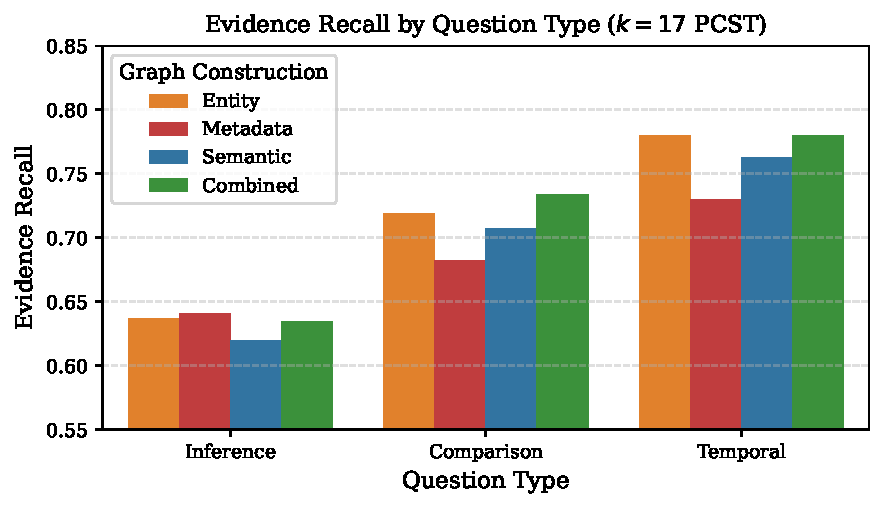
\includegraphics[width=\linewidth]{figures/fig_qtype_breakdown.pdf}
  \caption{Evidence recall by question type under default PCST settings ($k{=}17$).}
  \label{fig:qtype-breakdown}
\end{figure}

\end{document}
